

\chapter{Elektronik}
\label{chap:elektronik}

\section{Das Gehirn des Bootes}
Für die Steuerung des Bootes wird ein Raspberry Pi Zero W 1.1 verwendet. Dieser verfügt über ausreichend Leistung um alle notwendigen Berechnungen in Echtzeit durchzuführen. Auf dem Rasperry Pi läuft ein Debian basiertes GNU/Linux Betriebssystem. Im Kapitel Autonomie wird auf die Software jedoch genauer Eingeangen.

\begin{figure}
    \centering
    \includegraphics[width=0.5\linewidth]{assets/raspi Zero.jpg}
    \caption{Raspberry Pi Zero W}
    \label{fig:enter-label}
\end{figure}




\section{Sensoren und Aktuatoren}
\subsection{GPS}
Zur Bestimmung des aktuellen Standorts wird das Modul Neo 7M von Whadda verwendet. Dieses ist über eine Serielle Verbindung (RX und TX pins) verbunden.
\begin{figure}[H] 
    \centering
    \includegraphics[width=0.5\linewidth]{gps.png}
    \caption{GPS Modul}
    \label{fig:gps}
\end{figure}

\subsection{Gyro und Magnetometer}
Ein Magnetormeter wird als Kompass verwendet. Hierfür wird das Sensormodul GY-273 QMC5883L. Dieses Misst das Dreisimensionale Magnetische Feld aus welchem sich dann die Bootsrichtug ableiten lässt. Das Modul hat hat zudem ebenfalls einen Integrietes Gyroskop, somit ist ebenfalls möglich die Bewegung des Schiffes nachzuvollziehen und Schräglagen nachzuvollziehen. 

\begin{figure}[H]
    \centering
    \includegraphics[width=0.25\linewidth]{assets/magnetometer.jpg}
    \caption{Gyro und Magnetometer}

\end{figure}
\subsection{Aktuatoren}
Für die Bewegung des Ruders und des Sailflaps werden L16-100-63-6-R Aktuatoren von Actuonix verwendet. Diese sind für den Robotik ausgelegt und wasserdicht, was sie für diese Anwendung perfekt macht. Mit 6V (und 5V) können sie betrieben werden und haben eine 63:1 Übersetzung. Dies macht sie nicht besonders schnell, aber sie verfügen über die notwendige Kraft.
Sie verfügen über kein digitales Positionsfedback, dass heisst, dass nicht abgefragt werden kann, an welcher Position sich der "Stab" gerade befindet. Es können jedoch konkrete Distanzen angesteuert werden. Verbunden wird der Aktuator mit dem Pluspol und einer über das System geteiltem Ground. Über eine einzige Datenverbindung können kurze Impulse zwischen 1ms-2ms gesendet werden, wobei 1ms den Aktuator in die Startposition führt und der Aktuator bei 2ms voll ausgefahren wird. Um Einstellungen dazwischen zu erhalten, wird ein Wert zwischen 1ms und 2ms gesendet.  


?? HAST DU WATT ANGABEN???
\begin{figure}[H] 
    \centering
    \includegraphics[width=0.5\linewidth]{actuonix.png}
    \caption{Actuonix Aktuator}
    \label{fig:actuator}
\end{figure}


\subsection{Eiegenentwicklung des Windrichtungssensor}
Auf dem Markt gibt es erstaunlich wenige Windrichtungsmesser welche für dieses Projekt anwendbar wären. Manche sind zu gross, manche brauchen Energiemengen welche mir auf einem Boot nicht zur Verfügung stehen und wiederum andere sind schlichtweg zu teuer. Daher wird ein möglichst effizienteren jedoch kostengünstigen Sensor entwicket.
Populär sind vorallem zwei typen von Windrichtungssensoren, welche eine unterschiedliche Angehensweise haben, die Richtung des Windes digital festzuhalten. \\
Zum einen wären das Sensoren welche mithilfe eines Pontiometer funktionieren. Diese sind mechanisch sehr leicht umzusetzen, da man lediglich einen kleinen flügel an einem Potentiometer befestigt. Die Position kann in der Regel über einen Analogen Input pin auf einem Microcontroller eingelesen werden.
\\
Die zweite Option sind Hall Sensoren, mit welchen man typischerweise Stärke von Magneten misst. Um die Rotation eines Objektes mittels hallsensoren festzustellen gibt es 2 Möglichkeiten. Bei der ersten Variante plaziert man um ein abwechselnd magnetisch positiv und magnetisch positiv geladenes rundes Objekt eine belibige Anzahl an Hall sensoren um somit die Rotation zu messen. Das Problem dieser Methode ist die Vielzahl an benötigten Hallsensoren welche sehr aufwändig zu plazieren wären. Die Zweite und deutlich veilversprechendere Option sind sogenannten Rotary Hall Sensors. Hier wir ein AS5040-ASST Chip auf einen Adapterboard verwendet. Dies ermöglicht es den Windrichtungsmesser einfacher zusammen zu bauen.


\section{Energieversorgung}

Rechner, Sensoren und Aktuatoren werden mit elektrischer Energie betrieben. Weil das Segelboot vollkommen autonom funktionieren soll, muss diese auf dem Schiff selbst gewonnen werden. In Frage kommen dabei grundsätzlich drei Energiequellen, nämlich Wasserenergie, Windenergie und Sonnenenergie. 

\subsection{Wasserturbine}
Da sich das Boot im Wasser bewegt, könnte eine kleine Wasserturbine am Bootskörper befestigt und die Strömung zu deren Antrieb genutzt werden. Da sich das Boot relativ zum Wasser bewegt, gelten die gleichen Prinzipien wie bei Generierung elektrischer Energie durch Wasserkraft in Fliessgewässern.

Diese Methode hat jedoch gewichtige Nachteile. Segelboote erreichen, abgesehen von speziellen Konstruktionen wie sog. Foilingboote, bei denen der Bootskörper bei Fahrt vollständig aus dem Wasser gehoben wird, nur bescheidene Geschwindigkeiten. Da die Leistung einer Turbine in einer Flüssigkeit bei gleicher Fläche kubisch zur Strömungsgeschwindigkeit ansteigt, erlaubt diese Methode selbst bei idealen Segelbedingungen nur eine geringe Energieausbeute. Zudem würde das Segelboot durch die Turbine empfindlich abgebremst. 

\subsection{Windturbine}
Auch die Generierung von elektrischer Energie mithilfe einer Windturbine unter Nutzung der Windkraft ist nicht praktikabel. Um die Windenergie in Bewegungsenergie umzusetzen, aus der dann elektrische Energie generiert werden kann, muss ein Windrad in den Wind gedreht werden. Ein Segelboot kann keinen Kurs gegen den Wind segeln. Der Kurs vor dem Wind (also ein Kurs, bei dem der Wind von hinten auf das Boot trifft) ist zwar möglich, aber wenig effizient. Ein Windrad könnte folglich nicht fix mit dem Boot verbunden werden, sondern müsste drehbar ausgelegt werden, damit es unabhängig vom Kurs des Bootes in den Wind gedreht werden kann. Es müsste so platziert werden, dass nicht nur eine Berührung des Segels, sondern auch eine Berührung der Wasseroberfläche bei einer Kränkung (Schieflage) des Bootes ausgeschlossen ist. Damit müsste es am äussersten Bug, am äussersten Heck oder auf dem Mast platziert werden. Alle Positionen verbieten sich, da damit die Balance des Bootes akut gefährdet wäre. 

Schliesslich würde eine Positionierung am Bug oder Heck, je nach vorherrschendem Wind, zu einer vollen oder teilweisen Abschattung des Windrades durch das Segel oder des Segels durch das Windrad führen. Eine Positionierung auf dem Mast würde selbst im Fall eines Vertikalwindrades zu Verwirbelungen führen, welche die Segeleigenschaften des Bootes negativ beeinträchtigen würden. 

Einfluss auf den Kurs, da das Boot nicht verankert ist. Damit geht Energie verloren, da das Boot „weggeschoben“ wird, statt die Windenergie in nutzbare Drehung umzutzen.

\subsection{Photovoltaik}
Für die Nutzung der Sonnenenergie kommt nur die Methode der Photovoltaik in Frage. Die für den Betrieb von Wärme-Kraft-Maschinen erforderlichen Temperaturen lassen sich auf einem beweglichen Boot mit Sonnenenergie nicht erreichen.

Die Energieerzeugung mittels Photovoltaikanlagen ist auf Segelbooten bliebt und verbreitet. Solche Anlagen haben keinen Einfluss auf die Segeleigenschaften des Bootes. Die Energieausbeute hängt aber stark vom Sonnenstand und dem vorherrschenden Wetter ab. Im Gegensatz zu stationären Anlagen lassen sich Photovoltaikanlagen auf Booten nicht ideal auf die Sonne ausrichten und können je nach Kurs sogar vom Segel beschattet werden. Da während der Nachstunden überhaupt keine Energie gewonnen werden kann, muss das Boot zur Überbrückung zwingend mit einem Energiespeicher ausgerüstet werden.

\begin{itemize}
    \item Montage segel vs deck
    \item deck einfacher weil flach
    \item auswahl des Panels
    \item Grössenbeschränkung
    \item anforderungen an Laistungd es Panels
    \item Kompellt panel gekauft
    \item USB ausgang 5V
    \item Kostengünstig
    \item Outdoor einsatz Mobil entworfen worden das panel = Robust


\end{itemize}

\subsection{Enegiespeicher}
Während der Nachtstunden kann mit dem Solarpaneel keine Energie gewonnen werden kann und bei Nebel ist die Energieausbeute sehr gering. Daher muss das Boot zur Überbrückung dieser Phasen mit einem Energiespeicher ausgerüstet werden, damit seine Autonomie sichergestellt ist.

Es wurde vorgesehen, dass die Energiereserve einen Betrieb während drei Tagen (72 h) erlauben soll. Der genaue Energieverbrauch des Rechners, der Sensoren und vor allem der Aktuatoren hängt stark davon ab, wie oft Steuereingriffe vorgenommen werden müssen und Messdatenerfassungen, Neuberechnungen erfolgen. Es lässt sich daher nicht präzis berechnen, sondern nur abschätzen. 

Der Schätzwert für den Gesamtenergieverbrauch pro Stunde beträgt 1.5 Watt (bei 5 Volt Gleichspannung). Das ergibt einen Energieverbrauch von 36 Wattstunden pro Tag (24 h). Zur Überbrückung der vorgesehenen drei Tagen ohne Energiezufuhr muss der Speicher daher über eine Kapazität von mindestens 108 Wattstunden verfügen. 

Eine völlige Erschöpfung des Energiespeichers kann diesen schädigen, und muss daher verhindert werden. Aber bereits ein Absinken der Ladung auf unter 20 Prozent verkürzt dessen Lebensdauer. die Kapazität muss daher erhöht werden. Um über ausreichen Reserven zu verfügen, wird daher eine Kapazität von 185 Wattstunden vorgesehen.

Im Handel erhältliche sogenannte Powerbanks verfügen über eine Kapazität von bis zu 20'000 mAh, was eine Leistung von 100 Wh ergibt. Eine solche Powerbank genügt den gestellten Anforderungen damit nicht. Auch eine Kombination mehrerer Powerbanks scheidet aus, weil heute angebotene Geräte nicht auf die sogenannten Durchgangsladung (pass‐through charging) ausgelegt sind. Sie können also nicht geladen werden, während ein Verbraucher Energie bezieht.  

Deutlich grössere Powerstations, die insbesondere für den Campingeinsatz vorgesehen sind, verfügen über deutlich grössere Kapazitäten und sind duchgangsladungsfähig. Sie sind aber meist auf Verbraucher ausgelegt, die mit 220 V Wechselspannung betrieben werden,sind meist weit über 10 Kg schwer und kosten über 1000 Franken. Sie scheiden daher ebenfalls aus.   

Es muss daher auf eine Eigenentwicklung zurückgegriffen werden. Gängig dafür sind 18650 Li-ion Zellen. Die verwendeten Zellen verfügen über eine Akku Kapazität von 2'500 mAh bei 3.7 V. 
Der Akku wird in zwei Teile unterteilet, welche untereinander Parallel Geschalten sind. So bleibt die Spannung die selbe, jedoch erhöt sich die Kapazität. Die beiden Teile werden dann Seriel miteinander Vebunden. Somit ergibt sich eine Spannung von 7.4V und 25000mAh. 

Die einzelnen Zellen werden untereinander mit einem Nickelband verbunden, welches mit einem Punktschweissgerät direkt auf den Zellen verankert ist. Spezialwekzeug musste gekauft weren




\begin{figure}[H]
    \centering
    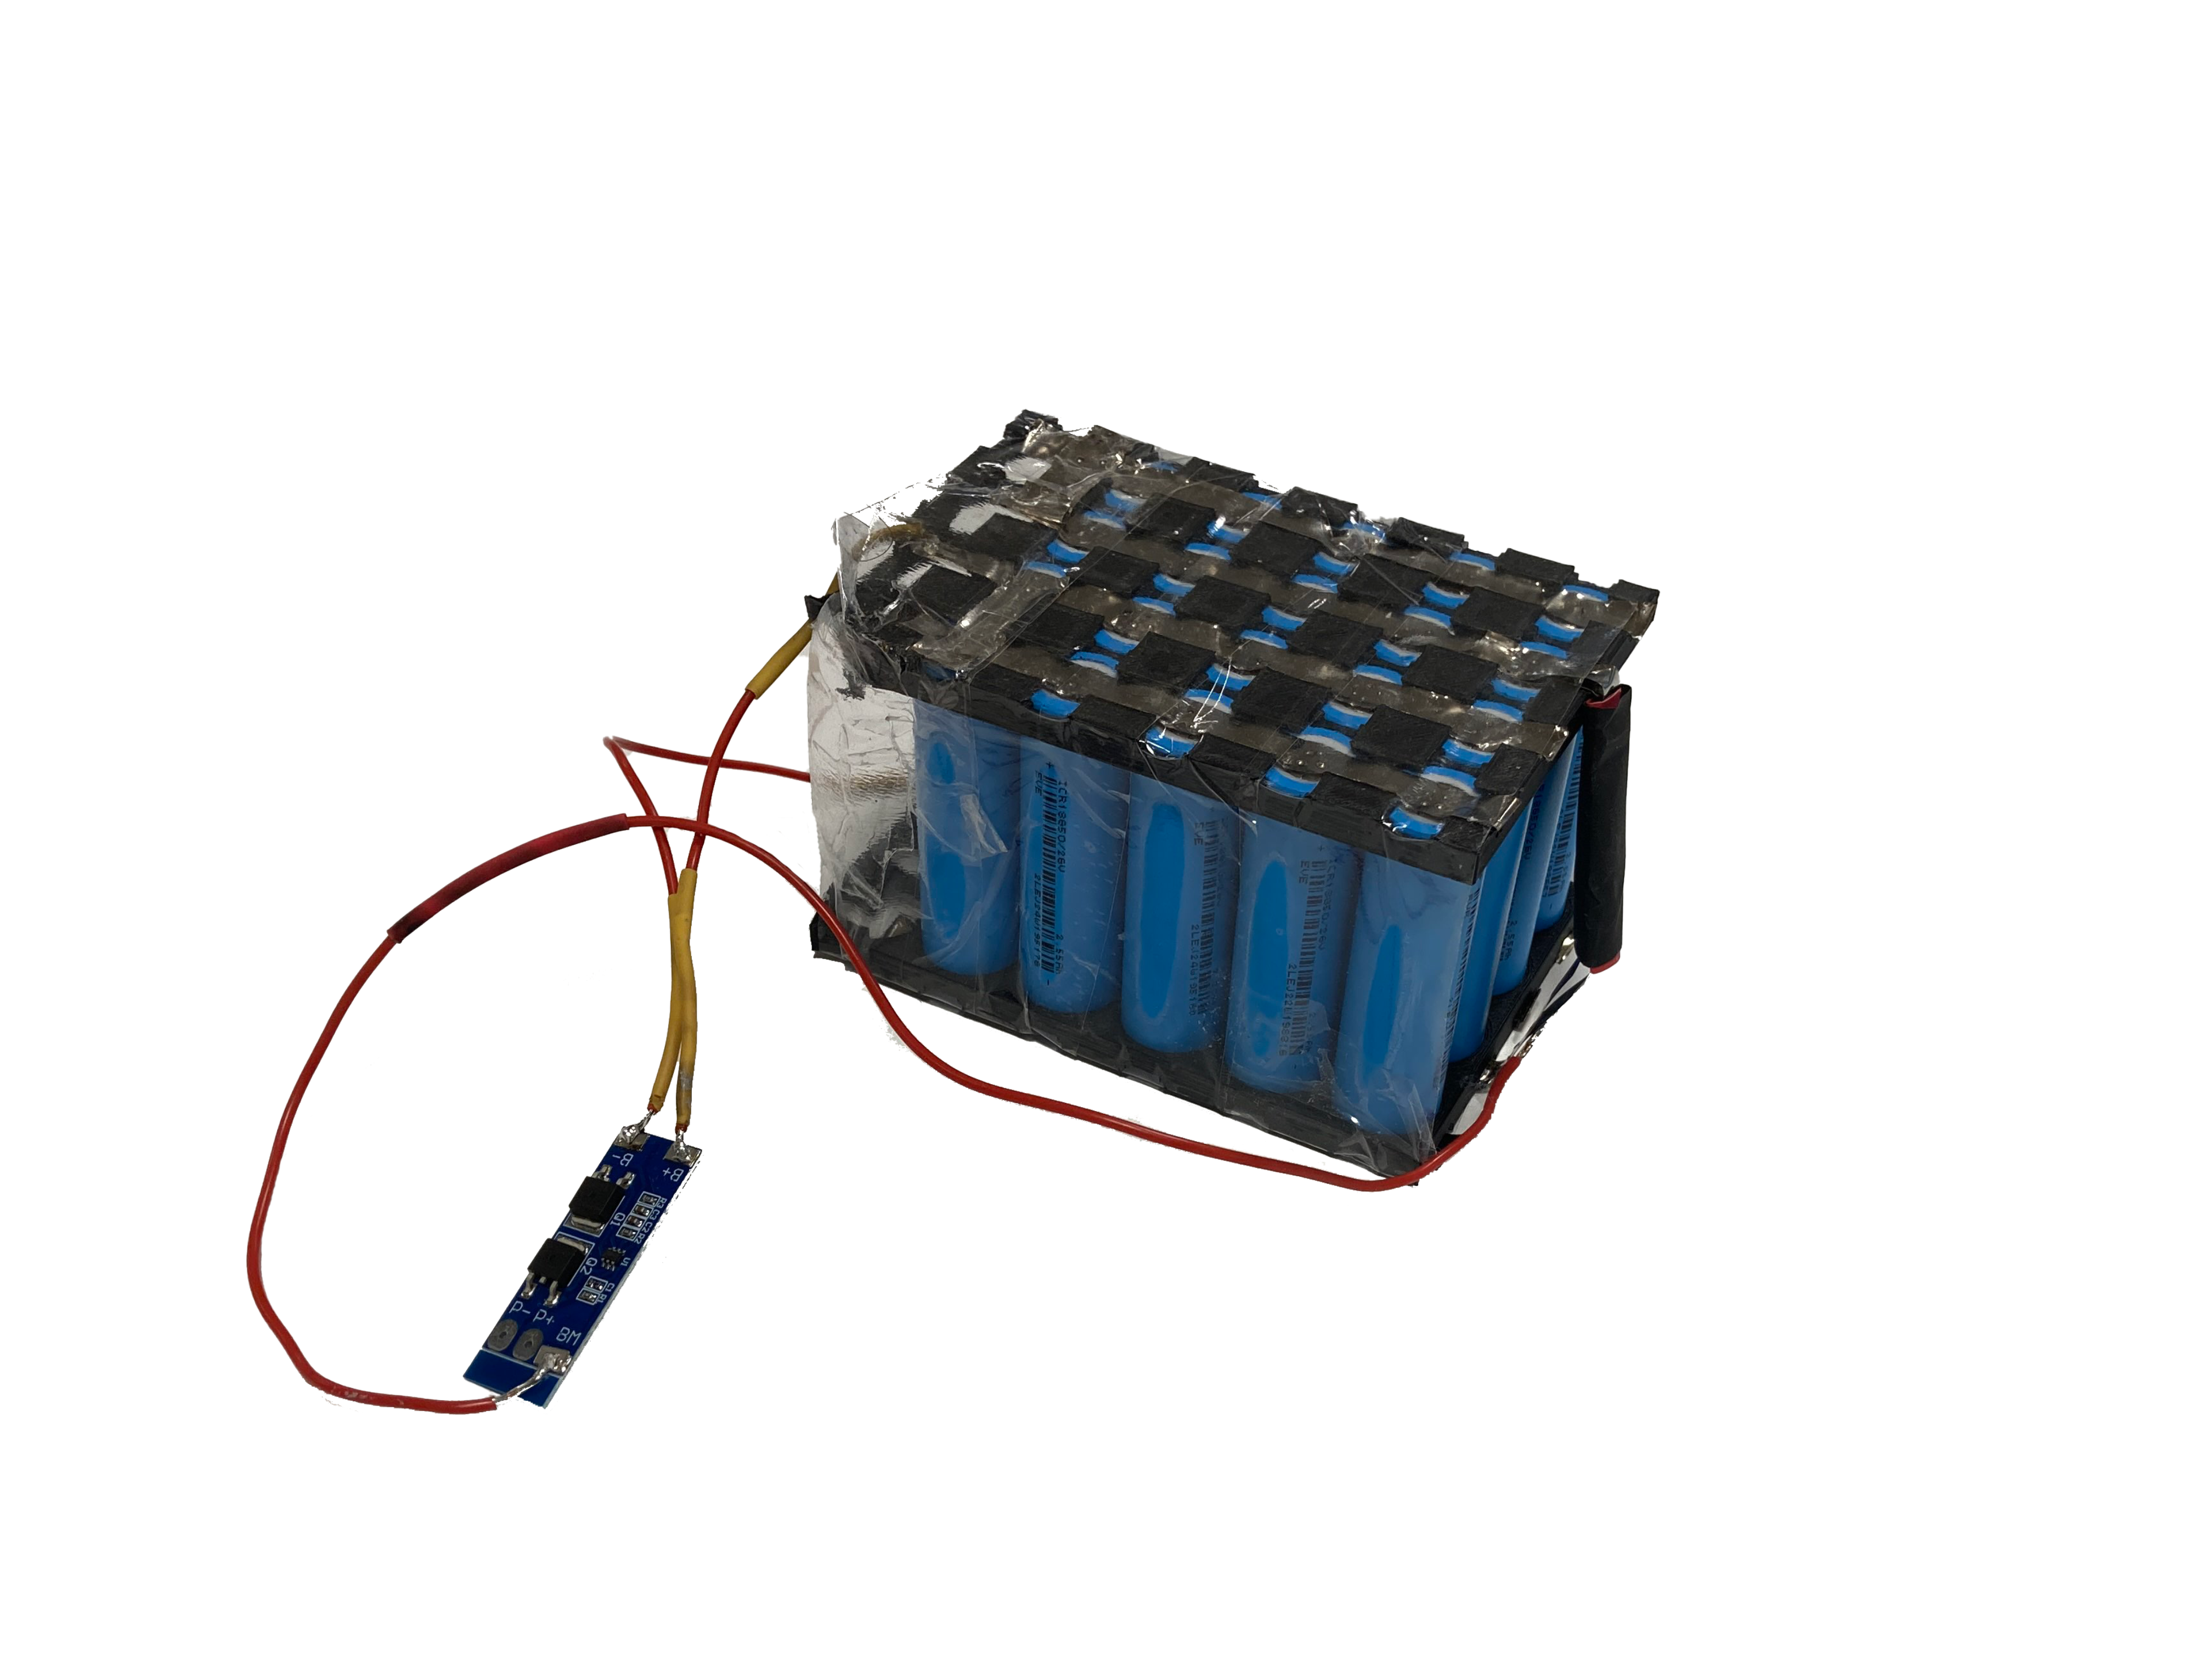
\includegraphics[width=0.75\linewidth]{assets/akku_transparent.png}
    \caption{Selbstgebauter Akku}
    \label{fig:enter-label}
\end{figure}


\subsection{Ladeeletronik und Spannungswandelung}

Da Litiumzellen beim einer überladung oder bei einer Entladung beschädigt oder im schlimmsten Fall in Flammen aufgehen, wird ein \ac{bms} verwendet. 

